% !TEX encoding = UTF-8 Unicode
\documentclass[portuguese, a4paper]{article}
\usepackage[margin=2.5cm]{geometry}
%\usepackage{fontspec} % XeLaTeX
\usepackage[T1]{fontenc} % LaTeX
\usepackage[utf8]{inputenc} % LaTeX
%\usepackage{newtxmath, newtxtext}
%\usepackage{lmodern}
\usepackage{csquotes}
\usepackage{babel}
%\usepackage[backend=bibtex]{biblatex}
%\usepackage[backend=biber]{biblatex}
%\addbibresource{bibliography.bib}

\usepackage{indentfirst}
\usepackage{graphicx}
	\graphicspath{{images/}}
\usepackage{grffile}
\usepackage{float}
\usepackage{amsmath}
	\allowdisplaybreaks
\usepackage{commath}
\usepackage{amssymb}
\usepackage{mathtools}
\usepackage{siunitx}
	\sisetup{inter-unit-product =\ensuremath{.}}
\usepackage{hyperref}

% Section styles
%\renewcommand{\thesection}{\Roman{section}}
%\renewcommand{\thesubsection}{\alph{subsection})}
%\renewcommand{\thesubsubsection}{\roman{subsubsection}.}
\renewcommand{\thesection}{}
\renewcommand{\thesubsection}{}
\renewcommand{\thesubsubsection}{}

% Useful commands
\newcommand{\eq}{\Leftrightarrow} % Equivalente
% Ordem de grandeza, e.g., "2\og{5}" => "2e5"
\newcommand{\og}[1]{{\times \num{e#1}}}
% Em um ponto, e.g. "f(x)\at{x=5}" = f(x)|x=5
\newcommand{\at}[1]{\left.\right|_{#1}}
% Para numerar apenas uma equação
\newcommand\numberthis{\addtocounter{equation}{1}\tag{\theequation}}
\DeclareMathOperator{\Div}{div}
\DeclareMathOperator{\Rot}{rot}
\newcommand{\real}{\ensuremath{\mathds{R}}}
 % Operator "d", e.g., "\frac{\dx{f}}{\dx{x}} = "df/dx"
\newcommand{\dx}[1]{\ensuremath{\operatorname{d}\!{#1}}}
\usepackage[overload]{abraces} % for curvy \overbrace

% Header and footer
\usepackage{fancyhdr}
\pagestyle{fancy}
\fancyhf{}
\lhead{Electrotecnia Teórica}
\rhead{1º Laboratório}
\lfoot{\small Engenharia Eletrotécnica e de Computadores - IST}
\rfoot{Página \thepage}
\renewcommand{\footrulewidth}{0.5pt}

% Document
\begin{document}
	\hypersetup{pageanchor=false}
	\begin{titlepage}
		\center
		\textsc{\bfseries\LARGE Instituto Superior Técnico}\\[1cm] % Name of your university/college
		
\includegraphics[height=1.5cm]{IST_Logo.pdf}\\[2.5cm]

		\textsc{\large Engenharia Eletrotécnica e de Computadores}\\[0.5cm] % Major heading such as course name
		\textsc{\Large Eletrotecnia Teórica}\\[0.5cm] % Minor heading such as course title
		\textsc{\large 2017/2018 2º Semestre}\\[2cm]

		\rule{\textwidth}{1.6pt}\vspace*{-\baselineskip}\vspace*{2pt} % Thick horizontal line
		\rule{\textwidth}{0.4pt}\\[\baselineskip] % Thin horizontal line
			\textsc{\Huge \bfseries 1º Trabalho Laboratorial}\\[0.2cm]
			\bigskip
			\textsc{\large \bfseries Determinação Experimental Da Matriz De Coeficientes De Capacidade De Um Sistema De N+1 Condutores \\
			(Via Analogia Reo-eléctrica)}\\[0.2cm]
		\rule{\textwidth}{0.4pt}\vspace*{-\baselineskip}\vspace{3.2pt} % Thin horizontal line
		\rule{\textwidth}{1.6pt}\\[5cm]

		\begin{minipage}{0.9\textwidth}
			\begin{flushleft} \large
				\begin{Large}\bfseries\textsc{Autores:}\end{Large}\\[0.4cm]
				\begin{tabular}{l l l}
					Ricardo Simões			& 70389 & \normalsize ricardo.f.d.simoes@ist.utl.pt \\
					Rita Ramos					& 81616 & \normalsize rita.ramos@tecnico.ulisboa.pt \\
					João Pinheiro				& 84086 & \normalsize joao.castro.pinheiro@tecnico.ulisboa.pt \\
					João Sebastião			& 84087 & \normalsize joaofpsebastiao@tecnico.ulisboa.pt \\
				\end{tabular}
			\end{flushleft}
		\end{minipage}\\[0.5cm]

		\large \bfseries Laboratório segunda-feira, 09h30-11h30, Grupo D\\
		\large 12 de março de 2018\\[1cm]
	\end{titlepage}
	\hypersetup{pageanchor=true}

	\section{Dimensionamento}
	\subsection{a)}
		\par
		Assumindo que a água é um meio linear, $\vec{J} = \sigma \vec{E}$, e que $\vec{E}$ e $\vec{J}$ são uniformes dentro do tanque, então:
		$$ U = RI \eq R = \dfrac{U}{I} = \dfrac{\int_{\tiny\overbrace[L1R]{(0)(4)}} \vec{E} \cdot d\vec{s}}{\int_{S_{(4)}}(\vec{J} \cdot \vec{n})dS} = \dfrac{aE}{\sigma Ewl} = \dfrac{a}{\sigma wl}$$
		\par
		Para determinar experimentalmente a condutividade $\sigma$ da água, mediremos $U$ e $I$, e então:
		$$ R = \frac{U}{I} = \dfrac{a}{\sigma wl} \eq \sigma = \frac{I}{U} \dfrac{a}{wl}$$

	\subsection{b)}
	\begin{figure}[h]
		\centering
		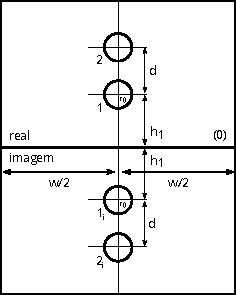
\includegraphics[width=0.4\linewidth]{imagem.pdf}
		\caption{Esquema para o método das imagens}
		\label{fig:imagem}
	\end{figure}

	\par
	Segundo a analogia reo-elétrica, é possível estabelecer uma relação entre a capacidade de um condensador e a condutância elétrica quando a geometria do sistema é idêntica.
	Sabe-se que na presença de uma corrente estacionária, a intensidade de corrente é dada por:

	\begin{align*}
		\int _ { S } \vec{J} \cdot \vec{n} d S = I
	\end{align*}

	\par
	Na situação do ensaio da figura 2, a intensidade do campo elétrico é constante e este é paralelo à normal, obtendo assim:

	\begin{align*}
		\vec{J} = \sigma \vec{E} \Rightarrow \int _ { S } \vec{J} \cdot \vec{n} d S = \int _ { S } \sigma \vec{E} \cdot \vec{n} d S  = \sigma E S = I
	\end{align*}

	\par
	Na presença de um campo elétrico estático, pela aplicação da Lei de Gauss, tem-se:

	\begin{align*}
			\int _ { S } \vec{D} \cdot \vec{n} d S = Q
	\end{align*}

	\par
	Do mesmo modo, devido ao facto de a intensidade do campo elétrico ser constante e paralelo à normal, tem-se:

	\begin{align*}
		\vec{J} = \epsilon \vec{E} \Rightarrow \int _ { S } \vec{D} \cdot \vec{n} d S = \int _ { S } \epsilon \vec{E} \cdot \vec{n} d S = \epsilon E S = Q
	\end{align*}

	\par
	Relacionando as expressões da capacidade de um condensador e condutância elétrica com as expressões obtidas acima, obtém-se:

	\begin{align*}
		\begin{cases}
			G = \dfrac{I}{U} = \dfrac{\sigma E S}{U} \\[1em]
    	C = \dfrac{Q}{U} = \dfrac{\epsilon E S}{U}
 		\end{cases}
	\end{align*}

	\begin{align*}
		\Rightarrow &\dfrac{G}{C} = \dfrac{I}{Q} = \dfrac{\sigma}{\epsilon} \Rightarrow Q = I\dfrac{\epsilon}{\sigma}
	\end{align*}

	\par
	Recorrendo ao método das imagens e usando a expressão obtida no laboratório inicial para o cálculo do potencial entre condutores filiformes, tem-se:

	\begin{align*}
		V_{ij} = \dfrac{q}{2\pi\epsilon} \ln\left(\dfrac{r'_{ij} }{r_{ij} }\right) = \dfrac{Q}{2\pi\epsilon l} \ln\left(\dfrac{r_{ij} '}{r_{ij} }\right)
	\end{align*}

	\par
	nde $r'_{ij}$ é a distância entre o condutor i e a imagem do condutor j e $r_{ij}$ é a distância real entre os condutores i e j. Por aplicação da Lei de Ohm e fazendo as respetivas substituições, obtém-se finalmente a expressão para calcular os elementos da matriz dos coeficientes de resistência para o sistema de condutores:

	\begin{align*}
		R_{ij} = \dfrac{V_{ij} }{I} &= \dfrac{\dfrac{Q}{2\pi\epsilon l} \ln\left(\dfrac{r'_{ij} }{r_{ij} }\right)}{I} = \\
		&= \dfrac{\dfrac{I\dfrac{\epsilon}{\sigma}}{2\pi\epsilon l}}{I} \ln\left(\dfrac{r'_{ij} }{r_{ij} }\right) = \\
		&= \dfrac{1}{2\pi\sigma l}\ln\left(\dfrac{r'_{ij} }{r_{ij} }\right)
	\end{align*}

	\par
	Esta matriz pode ser escrita na forma:

	\begin{align*}
		&[R] = \dfrac{1}{\sigma l} [K] \\
		&[K] = \dfrac{1}{2 \pi} \ln\left(\dfrac{r'_{ij} }{r_{ij} }\right)
	\end{align*}

	\par
	Onde $[K]$ depende apenas raio dos condutores cilíndricos e das distâncias destes entre si e ao plano condutor. Assim, com os dados fornecidos relativamente à posição relativa dos condutores, obtém-se a matriz $[K]$:

	\begin{align*}
		\begin{split}
		[K] &= \dfrac{1}{2\pi}
		\begin{bmatrix}
			\ln\left(\dfrac{2h_1}{r_0}\right) & \ln\left(\dfrac{2h_1 + d}{d}\right)  \\[1em]
			\ln\left(\dfrac{2h_1 + d}{d}\right) & \ln\left(\dfrac{2h_1 + d}{r_0}\right)
		\end{bmatrix} = \\
		&= \begin{bmatrix}
			0.547105466061146 & 0.239381352489734 \\
			0.239381352489734 & 0.619041132708855 \\
		\end{bmatrix}
		\end{split}
		\end{align*}

	\subsection{c)}

		\par
		Para calcular a matriz inversa de $[K]$, ou seja $[K]^{-1}$, recorreu-se ao Matlab, obtendo assim:

		\begin{align*}
			[K]^{-1} =
			\begin{bmatrix}
				2.200038917860650  & -0.850748462195038 \\
  				-0.850748462195038 & 1.944383424477395
			\end{bmatrix}
		\end{align*}

	\subsection{d)}

		\par
		Utilizando as matrizes calculadas anteriormente, sabe-se que:

		\begin{align*}
				&[U] = [R][I] \\
			\eq &[I] = [G][I] = \sigma l [K]^{-1}[I]
		\end{align*}

		\par
		Considerando $I = I_1 + I_2$ e $U_1 = U_2 = U$, retira-se:

		\begin{align*}
			I &= I_1 + I_2 = \sigma l \left[ \left(K^{-1}_{11}U_1 + K^{-1}_{12}U_2\right) + \left(K^{-1}_{21}U_1 + K^{-1}_{22}U_2\right) \right] \\
				&= \sigma l \left[ \left(K^{-1}_{11} + K^{-1}_{12}\right)U + \left(K^{-1}_{21} + K^{-1}_{22}\right)U \right] \\
				&= \sigma l \left( K^{-1}_{11} + K^{-1}_{12} + K^{-1}_{21} + K^{-1}_{22} \right) U\\ \\
			\Rightarrow U(I) &= \frac{I}{\sigma l \sum\limits_{i,j=1}^{2} K^{-1}_{ij}}
		\end{align*}

		\par
		Determinada a expressão de $U$ em função de $I$, é possível determinar a relação entre $I_1/I$ e $I_2/I$. Sabe-se, através da análise da equação matricial, que:

		\begin{align*}
				I_1 &= \sigma l \left(K^{-1}_{11}U_1 + K^{-1}_{12}U_2\right) = \sigma l \left(K^{-1}_{11} + K^{-1}_{12} \right)	U \Rightarrow \frac{I_1}{I} = \frac{K^{-1}_{11} + K^{-1}_{12}} {\sum\limits_{i,j=1}^{2} K^{-1}_{ij}} \\ \\
				I_2 &= \sigma l \left(K^{-1}_{21}U_1 + K^{-1}_{22}U_2\right) = \sigma l \left(K^{-1}_{21} + K^{-1}_{22} \right)	U \Rightarrow \frac{I_2}{I} = \frac{K^{-1}_{21} + K^{-1}_{22}} {\sum\limits_{i,j=1}^{2} K^{-1}_{ij}}
		\end{align*}



	\subsection{e)}
		\par
		O ensaio é realizado a $\SI{1}{\kilo\hertz}$ para evitar a eletrólise da água. Alternar o cátodo e ânodo sucessivamente, a uma frequência mais alta que a velocidade de reação da eletrólise, chegará para evitar a eletrólise e assim um aumento da temperatura da água, que influenciaria o valor da sua condutividade $\sigma$.

\end{document}
